\documentclass[aspectratio=169]{beamer}

\mode<presentation>
{
  \usetheme{default}
  \usecolortheme{default}
  \usefonttheme{default}
  \setbeamertemplate{navigation symbols}{}
  \setbeamertemplate{caption}[numbered]
  \setbeamertemplate{footline}[frame number]  % or "page number"
  \setbeamercolor{frametitle}{fg=white}
  \setbeamercolor{footline}{fg=black}
} 

\usepackage[english]{babel}
\usepackage[utf8x]{inputenc}
\usepackage{tikz}
\usepackage{courier}
\usepackage{array}
\usepackage{bold-extra}
\usepackage{minted}
\usepackage[thicklines]{cancel}
\usepackage{fancyvrb}

\xdefinecolor{dianablue}{rgb}{0.18,0.24,0.31}
\xdefinecolor{darkblue}{rgb}{0.1,0.1,0.7}
\xdefinecolor{darkgreen}{rgb}{0,0.5,0}
\xdefinecolor{darkgrey}{rgb}{0.35,0.35,0.35}
\xdefinecolor{darkorange}{rgb}{0.8,0.5,0}
\xdefinecolor{darkred}{rgb}{0.7,0,0}
\definecolor{darkgreen}{rgb}{0,0.6,0}
\definecolor{mauve}{rgb}{0.58,0,0.82}

\title[2018-07-12-chep-plenary-datamodels]{Data analysis tooling from within HEP and from industry}
\author{Jim Pivarski}
\institute{Princeton University -- DIANA-HEP}
\date{July 12, 2018}

\begin{document}

\logo{\pgfputat{\pgfxy(0.11, 7.4)}{\pgfbox[right,base]{\tikz{\filldraw[fill=dianablue, draw=none] (0 cm, 0 cm) rectangle (50 cm, 1 cm);}\mbox{\hspace{-8 cm}
\includegraphics[height=1 cm]{princeton-logo-long.png}
\includegraphics[height=1 cm]{diana-hep-logo-long.png}}}}}

\begin{frame}
  \titlepage
\end{frame}

\logo{\pgfputat{\pgfxy(0.11, 7.4)}{\pgfbox[right,base]{\tikz{\filldraw[fill=dianablue, draw=none] (0 cm, 0 cm) rectangle (50 cm, 1 cm);}\mbox{\hspace{-8 cm}
\includegraphics[height=1 cm]{princeton-logo.png}
\includegraphics[height=1 cm]{diana-hep-logo.png}}}}}

% Uncomment these lines for an automatically generated outline.
%\begin{frame}{Outline}
%  \tableofcontents
%\end{frame}

% START START START START START START START START START START START START START

\begin{frame}{}
\Large
\vspace{0.5 cm}
\begin{center}
I'm going to start with a dumb comparison, to make a point.
\end{center}
\end{frame}

\begin{frame}{\only<1>{We measure globally distributed data in hundreds of PB}\only<2>{But for ``web scale'' companies, 100 PB = 1 truck}}
\vspace{0.35 cm}
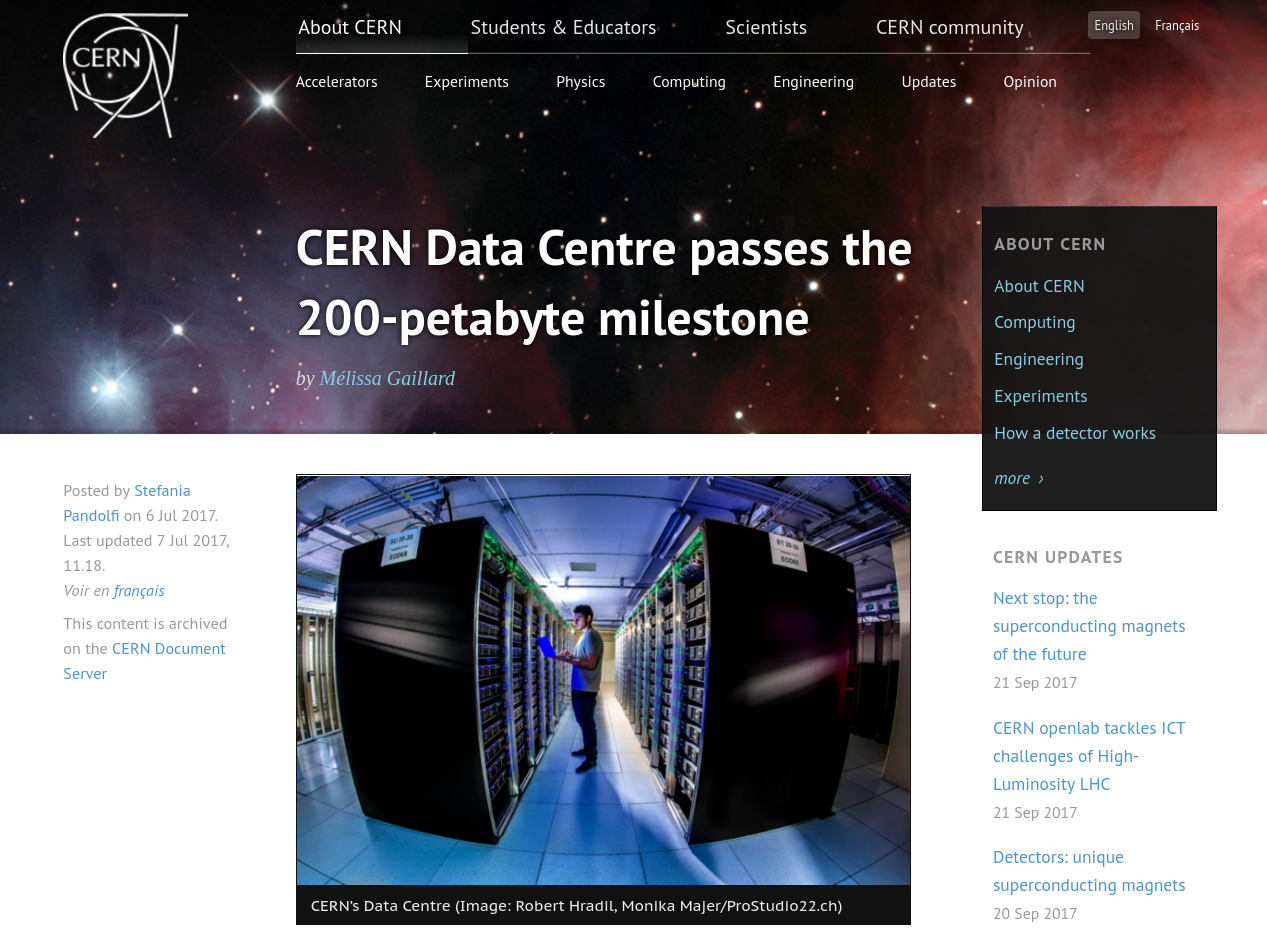
\includegraphics[width=0.73\linewidth]{cern-200pb.png}

\vspace{-4.8 cm}
\uncover<2->{\mbox{ } \hfill 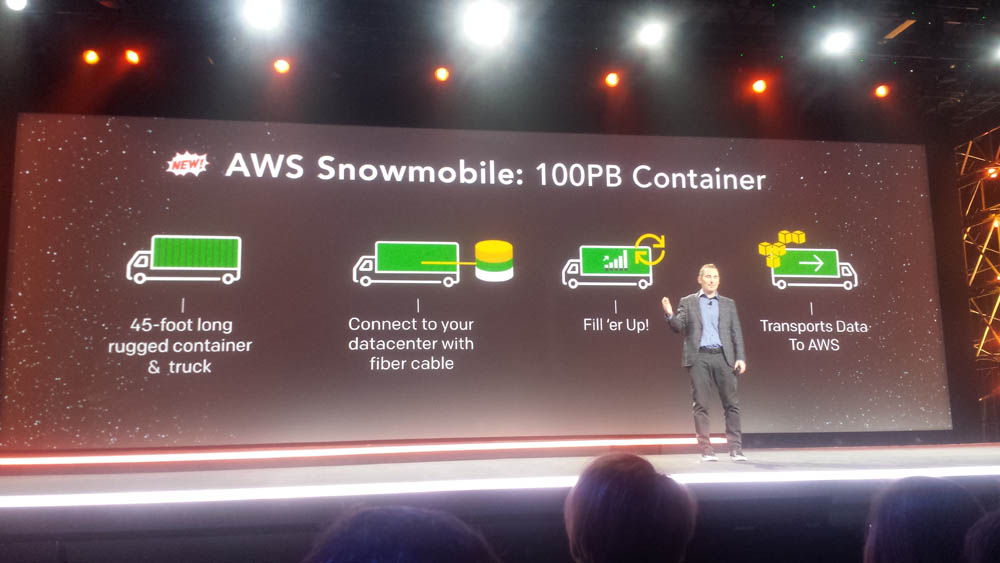
\includegraphics[width=0.7\linewidth]{aws-snowmobile.jpg}\hspace{-1 cm}}
\end{frame}

\begin{frame}{The point?}
\Large
\vspace{0.5 cm}
HEP is no longer the main user or developer in this problem space.

\vspace{1 cm}
\begin{uncoverenv}<2->
A better metric, which unfortunately I can't quantify:
\begin{itemize}
\item $x$~FTEs in HEP developing open source analysis tools
\item $y$~FTEs outside of HEP developing open source analysis tools
(not sure of $x$ and $y$, but $x \ll y$)
\end{itemize}
\end{uncoverenv}

\vspace{0.5 cm}
\uncover<3->{$\to$ there's a lot of good data analysis software out there!}
\end{frame}

\begin{frame}{Another very important metric}
\Large
\vspace{0.25 cm}
\begin{itemize}
\item High-energy physicists have been performing big data analytics (i.e.\ reducing large datasets to statistical inferences with computers) for about \textcolor{darkblue}{\underline{50~years}.}
\item<2-> Web-scale companies have been doing it for about \textcolor{darkblue}{\underline{10~years}.}
\end{itemize}

\vspace{0.5 cm}
\uncover<3->{HEP analyses have grown sophisticated--- there are certain things we expect but don't find in industry-grade software.}

\vspace{0.5 cm}
\uncover<4->{The simple prescription of ``just use Spark'' would leave analyzers}

\vspace{0.2 cm}
\uncover<4->{without some necessary tools.}
\end{frame}

\begin{frame}{Reactions?}
\large
\vspace{0.5 cm}
\begin{columns}[t]
\column{0.25\linewidth}
\textcolor{darkblue}{\underline{Option \#1}}

\vspace{0.25 cm}
All of our needs are specialized.

\vspace{0.25 cm}
Continue developing our own everything.

\vspace{1.75 cm}

\column{0.25\linewidth}
\begin{uncoverenv}<2->
\textcolor{darkblue}{\hspace{-0.18 cm}\underline{Option \#2}}

\vspace{0.25 cm}
Modern big data software has some good ideas; integrate those \underline{\it ideas} into our stack.
\end{uncoverenv}

\column{0.25\linewidth}
\begin{uncoverenv}<3->
\only<3-4>{\textcolor{darkblue}{\hspace{-0.18 cm}\underline{Option \#3}}}\only<5->{\textcolor{red}{\hspace{-0.18 cm}\underline{Option \#3}}}

\vspace{0.25 cm}
\only<3-4>{Narrow our scope to HEP-specific tools, what no one else is developing, and make them interoperate with non-HEP tools for the common parts.}\only<5->{\textcolor{red}{Narrow our scope to HEP-specific tools, what no one else is developing, and make them interoperate with non-HEP tools for the common parts.}}
\end{uncoverenv}

\column{0.25\linewidth}
\begin{uncoverenv}<4->
\textcolor{darkblue}{\hspace{-0.18 cm}\underline{Option \#4}}

\vspace{0.25 cm}
Convince the world to start using HEP analysis techniques so that they will develop solutions for these, too.
\end{uncoverenv}
\end{columns}

\vspace{1 cm}
\uncover<5->{\textcolor{red}{\#3 is my opinion, but it begs the question: what's HEP-specific?}}
\end{frame}

\begin{frame}{Three examples each:}
\Large
\vspace{0.5 cm}
\begin{columns}[t]
\column{0.5\linewidth}
\mbox{\hspace{0.25 cm}\underline{What they've got}}

\vspace{0.25 cm}
\begin{enumerate}
\item Distributed DAG processing
\item Indexed analysis
\item Machine learning
\end{enumerate}

\column{0.5\linewidth}
\mbox{\hspace{0.45 cm}\underline{What we'd need}}

\vspace{0.25 cm}
\begin{enumerate}
\item Nested data structures
\item Advanced histogramming
\item Ansatz fitting
\end{enumerate}

\end{columns}
\end{frame}

\begin{frame}{}
\huge
\vspace{0.5 cm}
\begin{center}
\textcolor{darkblue}{Distributed DAG processing}

\large
\vspace{0.5 cm}
not HEP-specific
\end{center}
\end{frame}

\begin{frame}{Distributed DAG processing}
\large
\vspace{0.5 cm}
\begin{columns}
\column{0.21\linewidth}
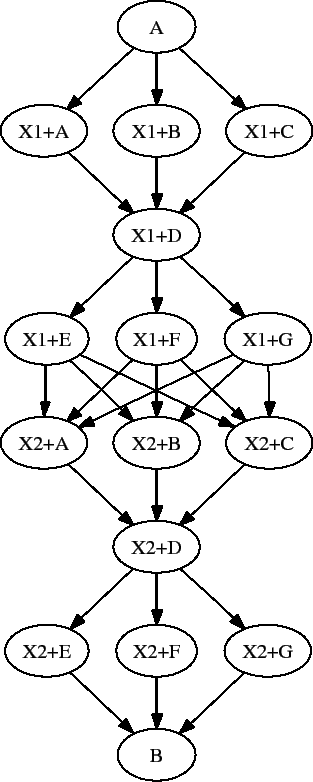
\includegraphics[width=\linewidth]{dag-htcondor.png}

\column{0.83\linewidth}
DAG: Directed Acyclic Graph of dependencies between subtasks.

In popular opinion, this is what big data processing \underline{\it is}.

\vspace{0.5 cm}
\begin{uncoverenv}<2->
Many frameworks distribute work this way:

\vspace{0.2 cm}
\hfill \begin{minipage}{0.95\linewidth}
\textcolor{darkblue}{Spark} (JVM), \textcolor{darkblue}{Dask} and \textcolor{darkblue}{Joblib} (Python), \textcolor{darkblue}{Storm} (continuous), \textcolor{darkblue}{Thrill} (C++), \textcolor{darkblue}{DAGMan} (HTCondor), \textcolor{darkblue}{TensorFlow} (ML)\ldots
\end{minipage}
\end{uncoverenv}

\vspace{0.5 cm}
\begin{uncoverenv}<3->
To use these frameworks, one must
\begin{itemize}
\item express user tasks as DAG nodes (e.g.\ ROOT RDataFrame);
\item serialize user functions on the driver and load user data on the workers in accordance to the framework's way of doing things.
\end{itemize}
\end{uncoverenv}

\vspace{0.5 cm}
\begin{uncoverenv}<4->
Spectrum of choices from ``bare Spark'' to ``reimplement Spark.''
\end{uncoverenv}
\end{columns}
\end{frame}

\begin{frame}{Distributed DAG processing}
\Large
\vspace{0.5 cm}
\begin{center}
However, most analysis needs for DAG processing are pretty simple: one level of {\tt\large map} (embarrassingly parallel event processing) and maybe one level of {\tt\large reduce} (combining aggregated data: {\tt\large hadd}).
\end{center}
\end{frame}

\begin{frame}{}
\huge
\vspace{0.5 cm}
\begin{center}
\textcolor{darkblue}{Nested data structures}

\large
\vspace{0.5 cm}
strangely HEP-specific
\end{center}
\end{frame}

\begin{frame}{Nested data structures}
\large
\vspace{0.5 cm}
\begin{columns}[t]
\column{0.5\linewidth}
\mbox{ } \hfill 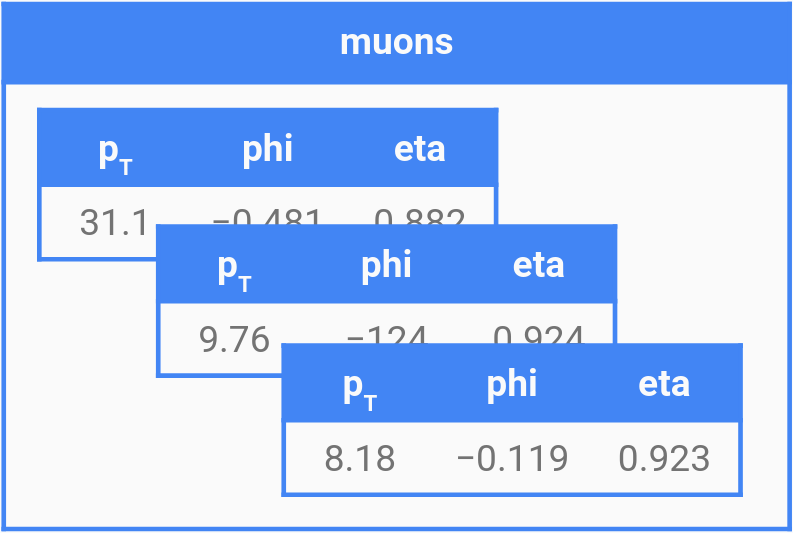
\includegraphics[width=0.75\linewidth]{muons-as-objects.png} \hfill \mbox{ }

\vspace{0.25 cm}
\begin{uncoverenv}<2->
Objects are essential in HEP analysis.

\vspace{0.25 cm}
Many physicists consider TTrees with {\tt\small std::vector<float>} branches to be ``minimal'' or ``flat.''
\end{uncoverenv}

\column{0.5\linewidth}
\mbox{ } \hfill 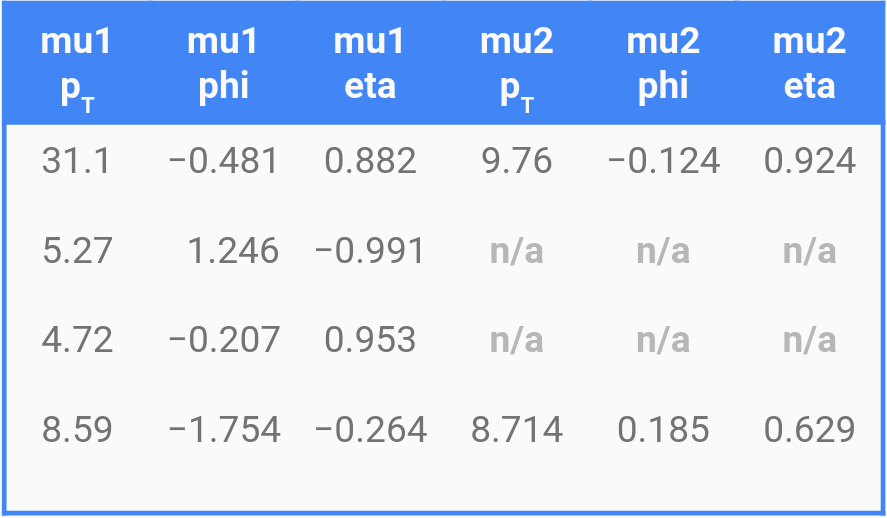
\includegraphics[width=0.75\linewidth]{muons-as-a-table.png} \hfill \mbox{ }

\vspace{0.25 cm}
\begin{uncoverenv}<3->
Most data analysis tools have an SQL mindset, with rectangular data tables.

\vspace{0.25 cm}
Objects $\to$ rectangular tables is a lossy conversion.

\vspace{0.25 cm}
Most performance claims start the stopwatch after this ``data cleaning.''
\end{uncoverenv}
\end{columns}
\end{frame}

\begin{frame}{Nested data structures}
\large
\vspace{0.5 cm}
{\Large ``But Spark/Parquet/Arrow/HDF5/Pandas allows nested objects!''}

\vspace{0.5 cm}
\uncover<2->{\textcolor{darkblue}{Nested data are included in the scope/data model, but are second-class citizens:}}

\vspace{0.25 cm}
\begin{itemize}\setlength{\itemsep}{0.25 cm}
\item<3-> \textcolor{darkblue}{Spark} DataFrames have arrays of structs, but using them involves a cumbersome explode-groupby or ``drop to RDDs,'' giving up performance.
\item<4-> \textcolor{darkblue}{Parquet} and \textcolor{darkblue}{Arrow} have lists of records, but they haven't been implemented in C++ and therefore Python yet (last time I checked).
\item<5-> \textcolor{darkblue}{HDF5} has lists of compound types, but not an efficient implementation.
\item<6-> \textcolor{darkblue}{Pandas} allows arbitrary Python objects in DataFrames, but most operations only apply to numbers.
\end{itemize}
\end{frame}

\begin{frame}[fragile]{Nested data structures}
\tiny
\vspace{0.25 cm}
\hfill 
\includegraphics[height=1 cm]{uproot-logo.pdf}

\vspace{-1.1 cm}
\begin{onlyenv}<1>\begin{minted}{python}
>>> import uproot
>>> t = uproot.open("tests/samples/HZZ.root")["events"]
>>> t.pandas.df(["MET_px", "Muon_Px", "Electron_Px"], entrystart=-20, flatten=False)
\end{minted}
\end{onlyenv}\begin{onlyenv}<2>\begin{minted}{python}
>>> import uproot
>>> t = uproot.open("tests/samples/HZZ.root")["events"]
>>> t.pandas.df(["MET_px", "Muon_Px", "Electron_Px"], entrystart=-20, flatten=True)
\end{minted}
\end{onlyenv}
\begin{onlyenv}<1>\begin{verbatim}
         MET_px                  Muon_Px              Electron_Px
2401   2.998099              [-1.492689]                       []
2402  27.944883              [-4.560287]                       []
2403   3.787466              [-9.715589]                       []
2404   9.378232             [-31.072098]                       []
2405 -17.310106   [47.484627, 4.6953125]                       []
2406 -81.965927   [74.75617, -20.911081]                       []
2407  -9.059591  [25.786427, -29.265024]                       []
2408  25.649775                       []                       []
2409  29.691553               [-24.7368]                       []
2410 -25.754967  [53.005814, -30.208649]  [-37.681973, 18.453588]
2411  -2.426847    [55.7203, -26.914448]                       []
2412 -15.611773              [14.896802]                       []
2413  18.921183             [-24.158083]                       []
2414 -11.730723              [-9.204197]                       []
2415 -10.648725   [34.506527, -31.56778]                       []
2416 -14.607650             [-39.285824]                       []
2417  22.208313              [35.067146]                       []
2418  18.101646             [-29.756786]                       []
2419  79.875191              [1.1418698]                       []
2420  19.713749              [23.913206]                       []
\end{verbatim}
\vspace{1.7 cm}
\end{onlyenv}\begin{onlyenv}<2>\begin{verbatim}
                   MET_px     Muon_Px  Electron_Px
entry subentry
2401  0          2.998099  -1.492689          NaN
2402  0         27.944883  -4.560287          NaN
2403  0          3.787466  -9.715589          NaN
2404  0          9.378232 -31.072098          NaN
2405  0        -17.310106  47.484627          NaN
      1               NaN   4.695312          NaN
2406  0        -81.965927  74.756172          NaN
      1               NaN -20.911081          NaN
2407  0         -9.059591  25.786427          NaN
      1               NaN -29.265024          NaN
2408  0         25.649775        NaN          NaN
2409  0         29.691553 -24.736799          NaN
2410  0        -25.754967  53.005814   -37.681973
      1               NaN -30.208649    18.453588
2411  0         -2.426847  55.720299          NaN
      1               NaN -26.914448          NaN
2412  0        -15.611773  14.896802          NaN
2413  0         18.921183 -24.158083          NaN
2414  0        -11.730723  -9.204197          NaN
2415  0        -10.648725  34.506527          NaN
      1               NaN -31.567780          NaN
2416  0        -14.607650 -39.285824          NaN
2417  0         22.208313  35.067146          NaN
2418  0         18.101646 -29.756786          NaN
2419  0         79.875191   1.141870          NaN
2420  0         19.713749  23.913206          NaN
\end{verbatim}
\end{onlyenv}

\vspace{-5 cm}
\hfill \begin{minipage}{0.33\linewidth}
\large
In some cases, maybe we're using the wrong idiom: instead of working with structured values, Pandas prefers structured indexes.
\end{minipage}
\vspace{5 cm}
\end{frame}

\begin{frame}[fragile]{Nested data structures}
\Large
\vspace{0.5 cm}
But that shouldn't be the only way: we {\it should} be able to use our data models and algorithms, even if we run them in workflow managers from the wider community.

\large
\vspace{0.5 cm}
\hfill 
\includegraphics[height=1 cm]{awkward-logo.pdf}

\vspace{-1 cm}
This is my main project: fast manipulation of columnar data.

\vspace{0.25 cm}
\scriptsize
\begin{columns}[t]
\column{0.35\linewidth}
\underline{\large General programming model}

\begin{minted}{python}
@numba.jit    # JIT-compiles Python
def deltaphi(event):
    metphi = event.MET.phi
    for jet in event.jets:
        yield metphi - jet.phi
\end{minted}

\column{0.45\linewidth}
\underline{\large Numpy-like broadcasting}

\begin{minted}{python}
# makes a copy of MET phi for each jet
event["MET"]["phi"] - event["jet"]["phi"]
\end{minted}
\end{columns}

\large
\vspace{0.5 cm}
This {\it ought} to be more general than HEP--- I'm in conversations with developers of Arrow, Dask, and XND ($\sim$Numpy 2.0) about these kinds of manipulations.
\end{frame}

\begin{frame}{}
\huge
\vspace{0.5 cm}
\begin{center}
\textcolor{darkblue}{Indexed analysis}

\large
\vspace{0.5 cm}
not well-known in HEP
\end{center}
\end{frame}

\begin{frame}{Indexed analysis}
\Large
\vspace{0.5 cm}
\begin{center}
To understand what I mean by ``indexed analysis,'' consider \\
analysis with \underline{\it less advanced indexing} than modern HEP.
\end{center}
\end{frame}

\begin{frame}[fragile]{Indexed analysis}
\vspace{0.1 cm}
\begin{columns}
\column{0.5\linewidth}
\tiny
\begin{Verbatim}[commandchars=\\\{\}]
h/cr/1d \textcolor{red}{201} 'd0miss' 100 -0.5e-3 0.5e-3
h/cr/1d \textcolor{red}{202} 'z0miss' 100 -0.015 0.015
h/cr/1d \textcolor{red}{203} 'pxmiss' 100 -0.076 0.076
h/cr/1d \textcolor{red}{204} 'pymiss' 100 -0.076 0.076
h/cr/1d \textcolor{red}{205} 'pzmiss' 100 -0.076 0.076
nt/plot 2.d0 ! ! ! ! ! \textcolor{red}{201}
nt/plot 2.z0 ! ! ! ! ! \textcolor{red}{202}
nt/plot 2.px ! ! ! ! ! \textcolor{red}{203}
nt/plot 2.py ! ! ! ! ! \textcolor{red}{204}
nt/plot 2.pz ! ! ! ! ! \textcolor{red}{205}

h/cr/1d \textcolor{red}{301} 'normalized d0miss' 100 -10 10
h/cr/1d \textcolor{red}{302} 'normalized z0miss' 100 -10 10
h/cr/1d \textcolor{red}{303} 'normalized pxmiss' 100 -10 10
h/cr/1d \textcolor{red}{304} 'normalized pymiss' 100 -10 10
h/cr/1d \textcolor{red}{305} 'normalized pzmiss' 100 -10 10
nt/plot 2.d0/sqrt(ed0) ! ! ! ! ! \textcolor{red}{301}
nt/plot 2.z0/sqrt(ez0) ! ! ! ! ! \textcolor{red}{302}
nt/plot 2.px/sqrt(epx) ! ! ! ! ! \textcolor{red}{303}
nt/plot 2.py/sqrt(epy) ! ! ! ! ! \textcolor{red}{304}
nt/plot 2.pz/sqrt(epz) ! ! ! ! ! \textcolor{red}{305}

h/cr/1d \textcolor{red}{401} 'd0miss after constraint' 100 -0.1e-16 0.1e-16
h/cr/1d \textcolor{red}{402} 'z0miss after constraint' 100 -0.1e-15 0.1e-15
h/cr/1d \textcolor{red}{403} 'pxmiss after constraint' 100 -0.01 0.01
h/cr/1d \textcolor{red}{404} 'pymiss after constraint' 100 -0.01 0.01
h/cr/1d \textcolor{red}{405} 'pzmiss after constraint' 100 -0.01 0.01
nt/plot 2.ad0 ! ! ! ! ! \textcolor{red}{401}
nt/plot 2.az0 ! ! ! ! ! \textcolor{red}{402}
nt/plot 2.apx ! ! ! ! ! \textcolor{red}{403}
nt/plot 2.apy ! ! ! ! ! \textcolor{red}{404}
nt/plot 2.apz ! ! ! ! ! \textcolor{red}{405}
\end{Verbatim}

\column{0.01\linewidth}

\column{0.5\linewidth}
To the left is a PAW script (pre-ROOT), creating and filling histograms.

\vspace{0.75 cm}
\textcolor{red}{They must be identified by integers because histograms didn't have \underline{\it names} back then.}

\vspace{0.75 cm}
\uncover<2->{{\bf Acquiring the ability to name stuff was as fundamental to HEP data analysis as handwashing was to medical science!}}

\vspace{0.75 cm}
\uncover<3->{But we don't have to stop there. There's more to indexing than key-value pairs.}
\end{columns}
\end{frame}

\begin{frame}{From ``Pandas DataFrames for F.A.S.T.\ binned analysis at CMS''}
\begin{center}
\only<1>{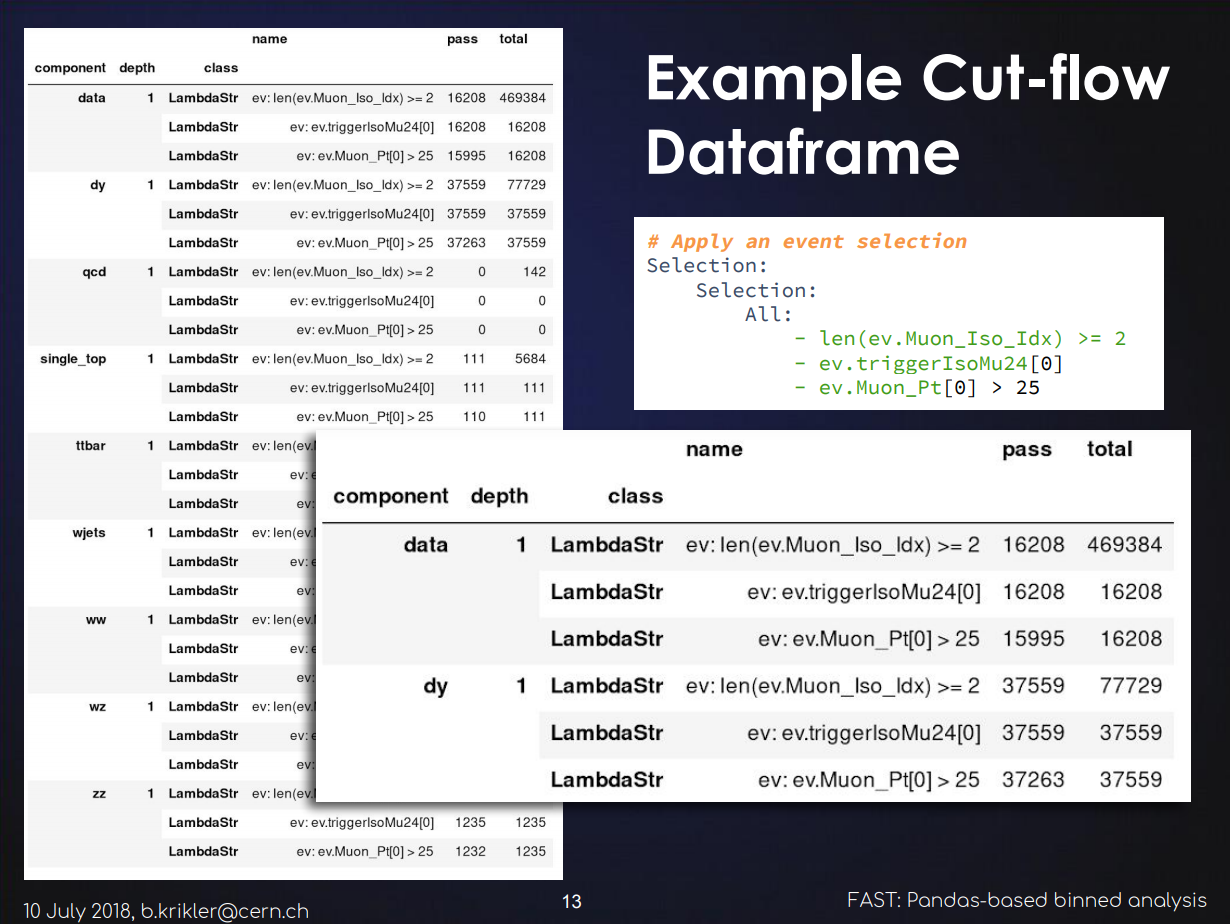
\includegraphics[width=0.75\linewidth]{fast-slide-0.png}}\only<2>{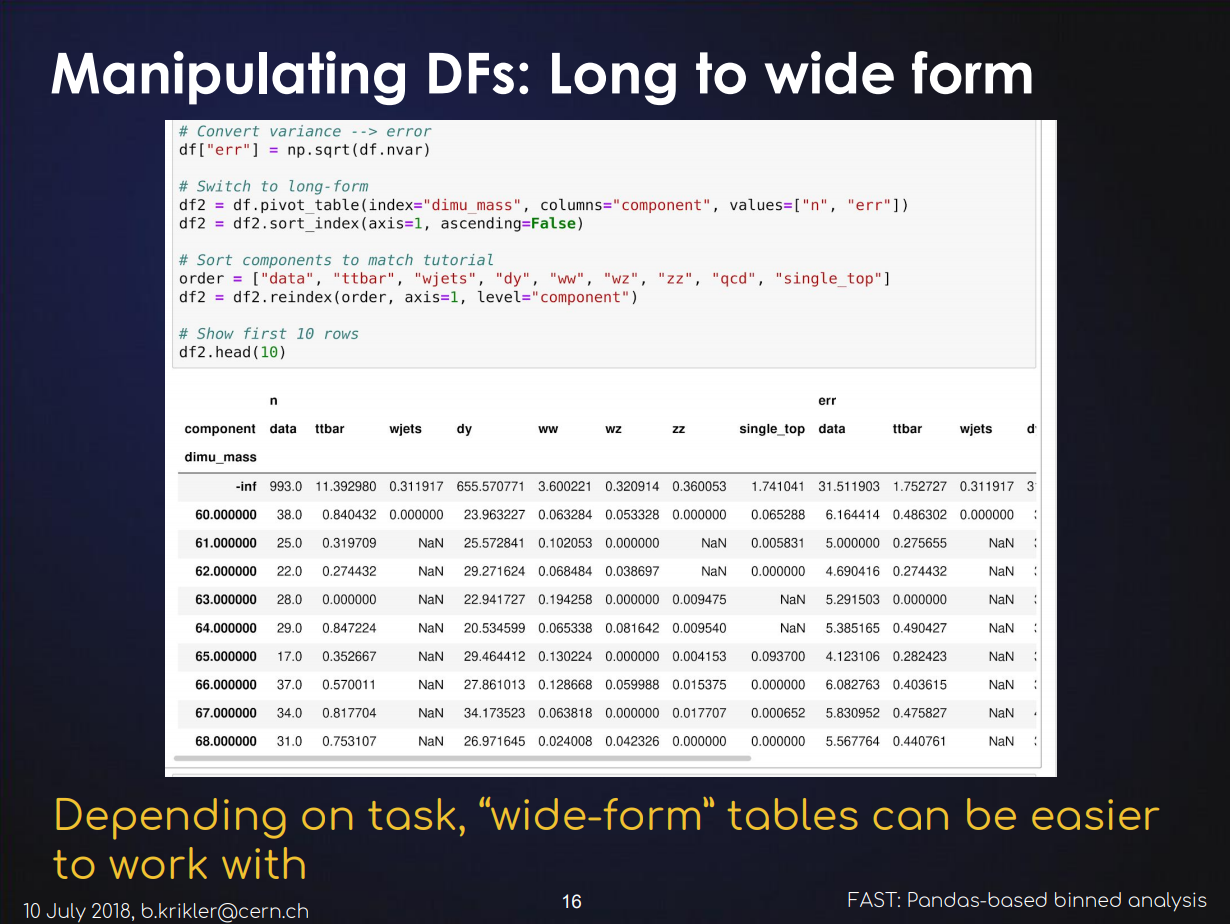
\includegraphics[width=0.75\linewidth]{fast-slide-2.png}}
\end{center}
\end{frame}

\begin{frame}[fragile]{Indexed analysis}
\large
\vspace{0.25 cm}
I had the same thought: our prime example of indexable data are histograms and systems of related histograms. Indexing would let us project/rebin/cut/transform histograms more fluidly.

\vspace{-0.5 cm}
\hfill 
\includegraphics[height=1 cm]{histbook-logo.pdf}

\vspace{-0.5 cm}
\vspace{0.25 cm}
\begin{onlyenv}<1>
\scriptsize
\begin{minted}{python}
>>> from histbook import *
>>> multihist = Hist(bin("mass", 100, 0, 500), cut("q1*q2 < 0"),
...                  split("mt1", [0.2, 0.5]), split("mt2", [0.2, 0.5]), fill=df)
>>> multihist.pandas()
\end{minted}
\tiny
\vspace{-0.25 cm}
\begin{verbatim}
                                                  count() err(count())
mass           q1*q2 < 0 mt1         mt2
[-inf, 0.0)    fail      [-inf, 0.2) [-inf, 0.2)      0.0          0.0
                                     [0.2, 0.5)       0.0          0.0
                                     [0.5, inf)       0.0          0.0
                         [0.2, 0.5)  [-inf, 0.2)      0.0          0.0
                                     [0.2, 0.5)       0.0          0.0
                                     [0.5, inf)       0.0          0.0
                         [0.5, inf)  [-inf, 0.2)      0.0          0.0
                                     [0.2, 0.5)       0.0          0.0
                                     [0.5, inf)       0.0          0.0
               pass      [-inf, 0.2) [-inf, 0.2)      0.0          0.0
                                     [0.2, 0.5)       0.0          0.0
                                     [0.5, inf)       0.0          0.0
                         [0.2, 0.5)  [-inf, 0.2)      0.0          0.0
                                     [0.2, 0.5)       0.0          0.0
                                     [0.5, inf)       0.0          0.0
                         [0.5, inf)  [-inf, 0.2)      0.0          0.0
                                     [0.2, 0.5)       0.0          0.0
\end{verbatim}
\end{onlyenv}
\begin{onlyenv}<2>
\scriptsize
\begin{minted}{python}
>>> from histbook import *
>>> multihist = Hist(bin("mass", 100, 0, 500), cut("q1*q2 < 0"),
...                  split("mt1", [0.2, 0.5]), split("mt2", [0.2, 0.5]), fill=df)
>>> multihist.step("mass")
\end{minted}
\mbox{ } \hfill 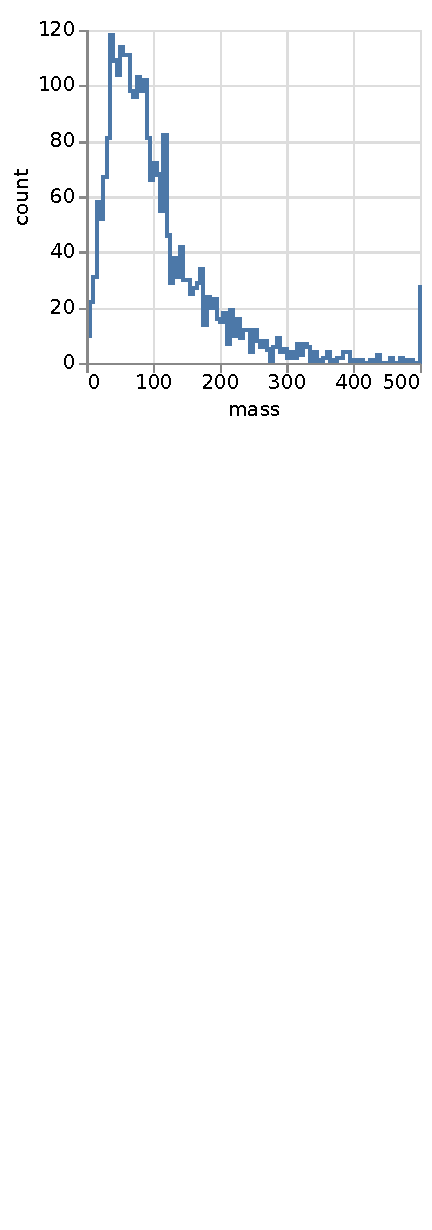
\includegraphics[height=7 cm]{pandhist.pdf} \hfill \mbox{ }
\end{onlyenv}
\begin{onlyenv}<3>
\scriptsize
\begin{minted}{python}
>>> from histbook import *
>>> multihist = Hist(bin("mass", 100, 0, 500), cut("q1*q2 < 0"),
...                  split("mt1", [0.2, 0.5]), split("mt2", [0.2, 0.5]), fill=df)
>>> multihist.overlay("q1*q2 < 0").step("mass")
\end{minted}
\mbox{ } \hfill 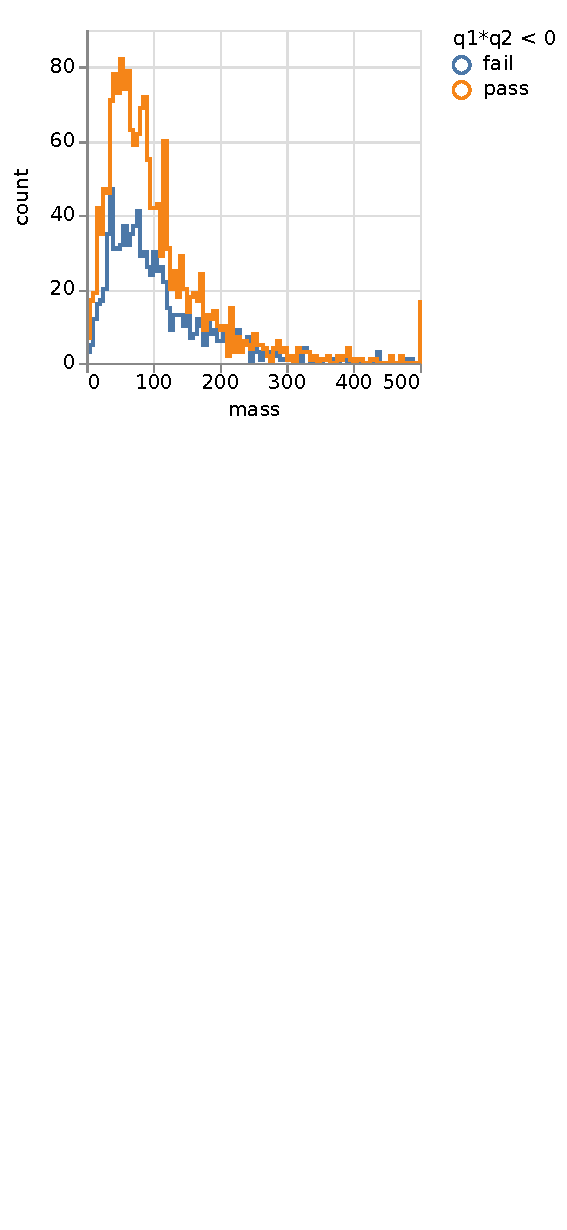
\includegraphics[height=7 cm]{pandhist_overlay.pdf} \hfill \mbox{ }
\end{onlyenv}
\begin{onlyenv}<4>
\scriptsize
\begin{minted}{python}
>>> from histbook import *
>>> multihist = Hist(bin("mass", 100, 0, 500), cut("q1*q2 < 0"),
...                  split("mt1", [0.2, 0.5]), split("mt2", [0.2, 0.5]), fill=df)
>>> multihist.stack("q1*q2 < 0").area("mass")
\end{minted}
\mbox{ } \hfill 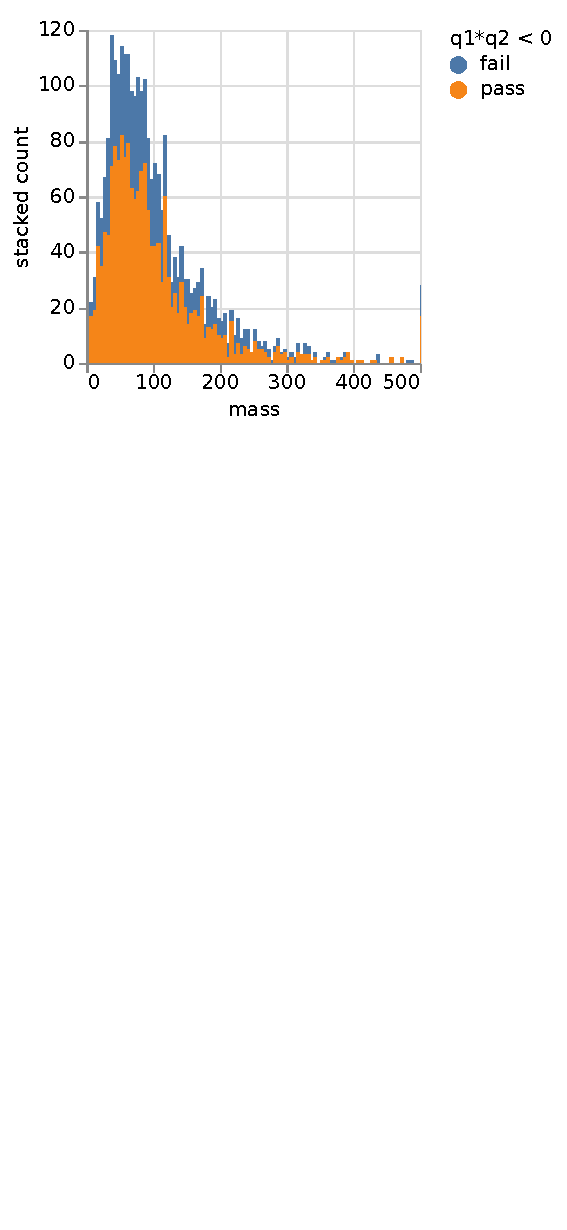
\includegraphics[height=7 cm]{pandhist_stack.pdf} \hfill \mbox{ }
\end{onlyenv}
\begin{onlyenv}<5>
\scriptsize
\begin{minted}{python}
>>> from histbook import *
>>> multihist = Hist(bin("mass", 100, 0, 500), cut("q1*q2 < 0"),
...                  split("mt1", [0.2, 0.5]), split("mt2", [0.2, 0.5]), fill=df)
>>> multihist.beside("q1*q2 < 0").step("mass")
\end{minted}
\mbox{ } \hfill 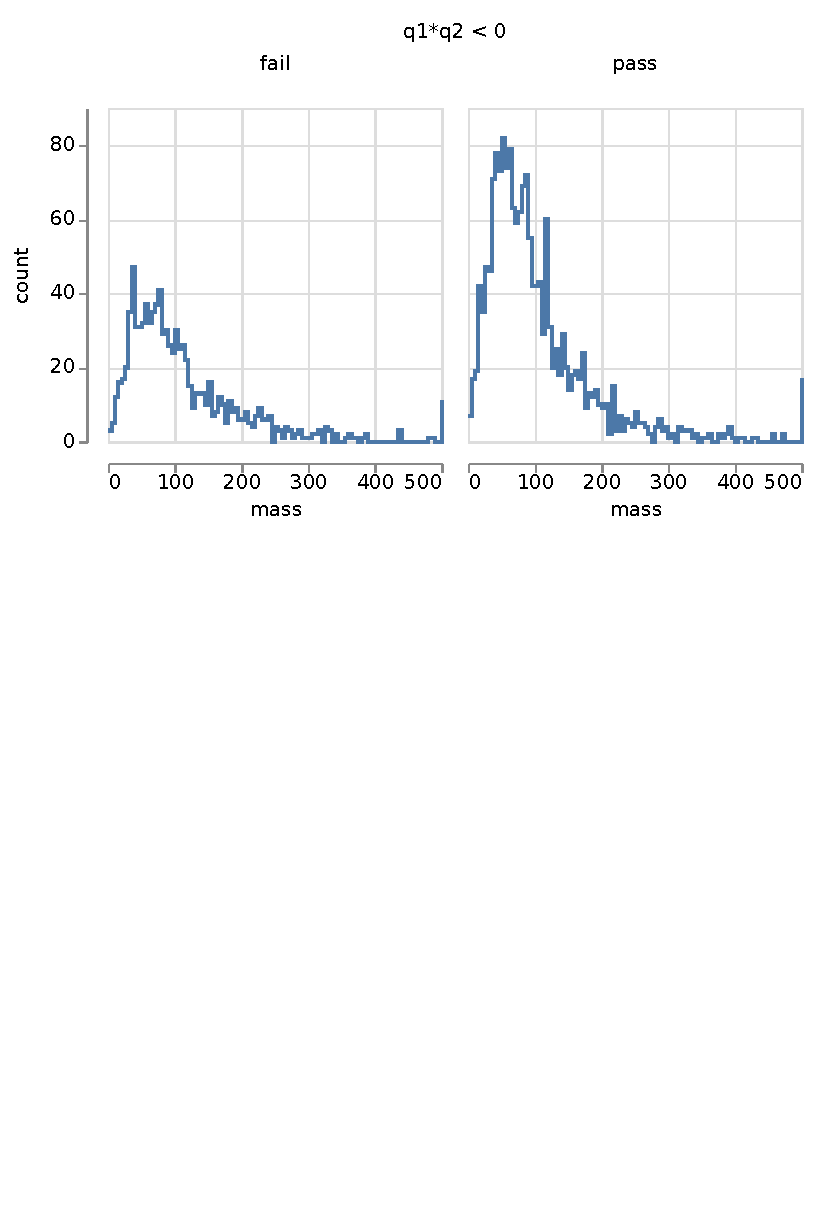
\includegraphics[height=7 cm]{pandhist_trellis.pdf} \hfill \mbox{ }
\end{onlyenv}
\begin{onlyenv}<6>
\scriptsize
\begin{minted}{python}
>>> from histbook import *
>>> multihist = Hist(bin("mass", 100, 0, 500), cut("q1*q2 < 0"),
...                  split("mt1", [0.2, 0.5]), split("mt2", [0.2, 0.5]), fill=df)
>>> multihist.below("mt1").beside("mt2").step("mass")
\end{minted}
\mbox{ } \hfill 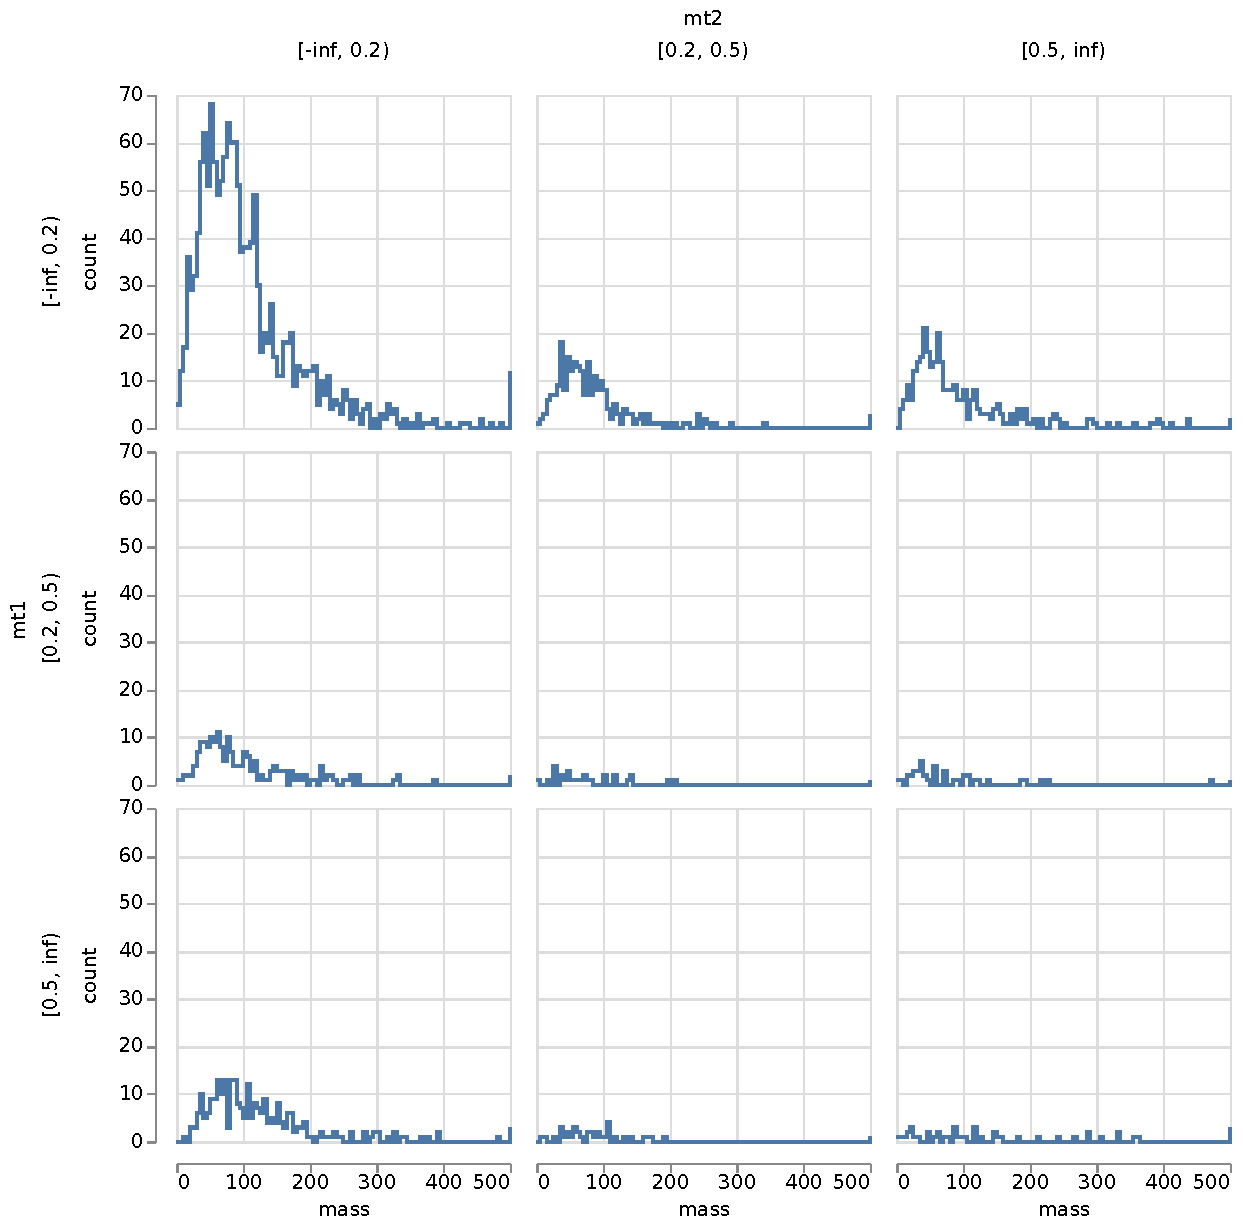
\includegraphics[height=7 cm]{pandhist_double_trellis.pdf} \hfill \mbox{ }
\end{onlyenv}
\begin{onlyenv}<7>
\scriptsize
\begin{minted}{python}
>>> from histbook import *
>>> multihist = Hist(bin("mass", 100, 0, 500), cut("q1*q2 < 0"),
...                  split("mt1", [0.2, 0.5]), split("mt2", [0.2, 0.5]), fill=df)
>>> multihist.below("mt1").beside("mt2").overlay("q1*q2 < 0").step("mass")
\end{minted}
\mbox{ } \hfill 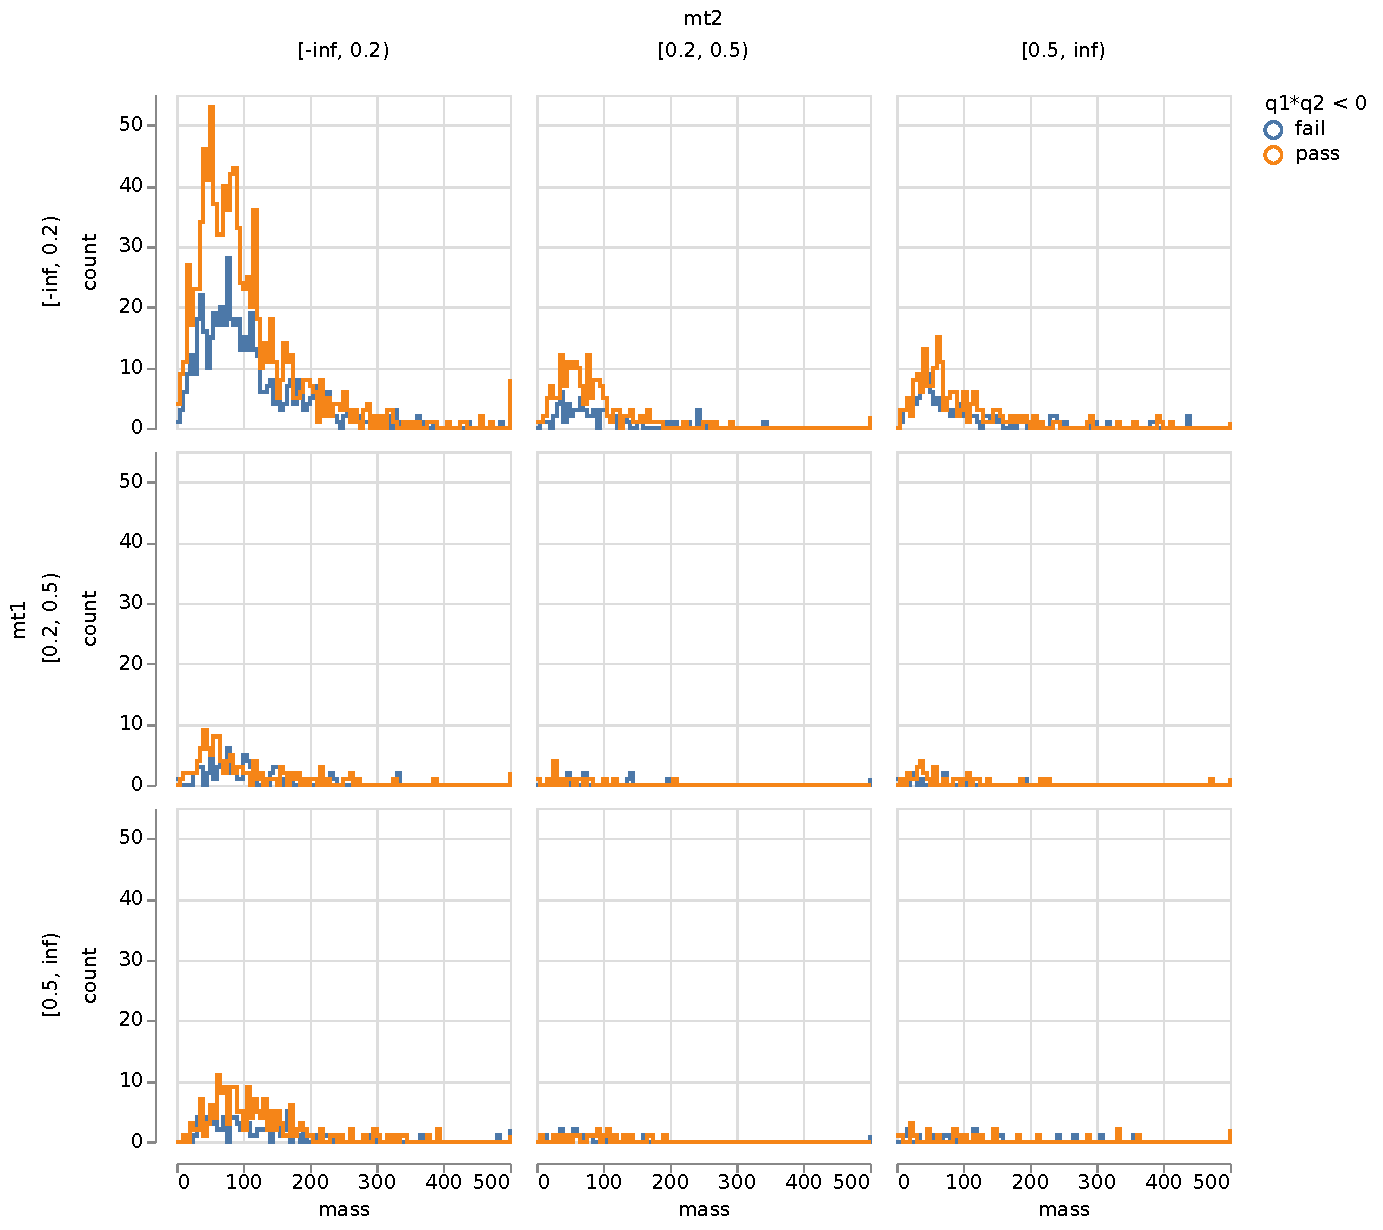
\includegraphics[height=7 cm]{pandhist_double_trellis_overlay.pdf} \hfill \mbox{ }
\end{onlyenv}
\end{frame}

\begin{frame}{Indexed analysis}
\Large
\vspace{0.5 cm}
Using tools with rich indexing systemizes what we're doing with naming conventions, splitting histogram names on underscores, etc.

\vspace{1 cm}
Pandas is not a TTree replacement--- if anything, it's a histogram organizer!

\vspace{1 cm}
\end{frame}

%% \begin{frame}[fragile]{Indexed analysis}
%% \vspace{0.1 cm}
%% \begin{columns}
%% \column{1.09\linewidth}
%% \begin{onlyenv}<1-2>Booking/filling mechanism with tree-like semantic index:

%% \hfill 
\includegraphics[height=1 cm]{histbook-logo.pdf}

%% \vspace{-1 cm}
%% \scriptsize
%% \begin{minted}{python}
%% >>> from histbook import *
%% >>> histograms = \
%% ...     ChannelsBook(
%% ...         mass = SamplesBook(["data", "signal", "background"],
%% ...                   SystematicsBook(Hist(bin("x", 5, 0, 5), systematic=[0]),
%% ...                                   Hist(bin("x + epsilon", 5, 0, 5), systematic=[1]),
%% ...                                   Hist(bin("x - epsilon", 5, 0, 5), systematic=[-1]))),
%% ...         mctruth = SamplesBook(["signal", "background"],
%% ...                         Book(param1=Hist(bin("param1", 5, 0, 5)),
%% ...                              param2=Hist(bin("param2", 5, 0, 5)))))
%% \end{minted}

%% \normalsize
%% defines $3\times 3 + 2\times2$ histograms and verifies that binning matches for systematic variations.

%% \scriptsize
%% \begin{uncoverenv}<2->
%% \begin{minted}{python}
%% >>> histograms.allkeys()
%% ['mass', 'mass/data', 'mass/data/0', 'mass/data/0/0', 'mass/data/0/1', 'mass/data/0/2',
%%  'mass/signal', 'mass/signal/0', 'mass/signal/0/0', 'mass/signal/0/1', 'mass/signal/0/2',
%%  'mass/background', 'mass/background/0', 'mass/background/0/0',  'mass/background/0/1',
%%  'mass/background/0/2', 'mctruth', 'mctruth/signal', 'mctruth/signal/0',
%%  'mctruth/signal/0/param2', 'mctruth/signal/0/param1', 'mctruth/background',
%%  'mctruth/background/0', 'mctruth/background/0/param2', 'mctruth/background/0/param1']
%% \end{minted}
%% \end{uncoverenv}
%% \vspace{-0.7 cm}
%% \end{onlyenv}
%% \begin{onlyenv}<3>
%% \scriptsize
%% \begin{minted}{python}
%% >>> print(histograms["mass"])                   # print just the "mass" channel
%% SamplesBook({
%%     'data': Book({
%%           '0': SystematicsBook({
%%                 '0': Hist(bin('x', 5, 0.0, 5.0)),
%%                 '1': Hist(bin('x + epsilon', 5, 0.0, 5.0)),
%%                 '2': Hist(bin('x - epsilon', 5, 0.0, 5.0))
%%                 })
%%           }),
%%     'signal': Book({
%%           '0': SystematicsBook({
%%                 '0': Hist(bin('x', 5, 0.0, 5.0)),
%%                 '1': Hist(bin('x + epsilon', 5, 0.0, 5.0)),
%%                 '2': Hist(bin('x - epsilon', 5, 0.0, 5.0))
%%                 })
%%           }),
%%     'background': Book({
%%           '0': SystematicsBook({
%%                 '0': Hist(bin('x', 5, 0.0, 5.0)),
%%                 '1': Hist(bin('x + epsilon', 5, 0.0, 5.0)),
%%                 '2': Hist(bin('x - epsilon', 5, 0.0, 5.0))
%%                 })
%%           })})
%% \end{minted}
%% \end{onlyenv}
%% \begin{onlyenv}<4>
%% \scriptsize
%% \begin{minted}{python}
%% >>> print(histograms.view("*/signal/*"))        # select the subtree matching this pattern
%% ViewBook({
%%       'mass': ViewBook({
%%             'signal': ViewBook({
%%                   '0': ViewBook({
%%                         '0': Hist(bin('x', 5, 0.0, 5.0)),
%%                         '1': Hist(bin('x + epsilon', 5, 0.0, 5.0)),
%%                         '2': Hist(bin('x - epsilon', 5, 0.0, 5.0))
%%                         })
%%                   })
%%             }),
%%       'mctruth': ViewBook({
%%             'signal': ViewBook({
%%                   '0': ViewBook({
%%                         'param2': Hist(bin('param2', 5, 0.0, 5.0)),
%%                         'param1': Hist(bin('param1', 5, 0.0, 5.0))
%%                         })
%%                   })
%%             })
%%       })
%% >>> histograms.view("*/data/*").fill(data)      # fill selectively
%% >>> histograms.view("*/signal/*").fill(signal)
%% >>> histograms.view("*/background/*").fill(background)
%% \end{minted}
%% \end{onlyenv}
%% \end{columns}
%% \end{frame}

\begin{frame}{}
\huge
\vspace{0.5 cm}
\begin{center}
\textcolor{darkblue}{Advanced histogramming}

\large
\vspace{0.5 cm}
very HEP-specific
\end{center}
\end{frame}

\begin{frame}{Advanced histogramming}
\large
\vspace{0.5 cm}
{\Large The histograms themselves, however, are more sophisticated in HEP than elsewhere.}
\vspace{0.25 cm}
\begin{itemize}\setlength{\itemsep}{0.25 cm}
\item<2-> As far as I have found, HEP histogramming tools (ROOT, YODA, AIDA, HippoDraw, Jas3, mn\_fit, PAW, HBOOK) are \underline{\it unique} in conceiving of a histogram as a container to be filled, merged, and accessed programmatically.
\item<3-> In many non-HEP packages, ``histogram'' is more of a display option than an analysis tool, with no way to access contents or control binning.
\item<4-> Only HEP tools have ``profile'' histograms--- functions of dependent variables, in addition to distributions on independent variables.
\item<5-> Log-scale support is often weak in non-HEP graphics packages, particularly for empty bins.
\end{itemize}
\begin{center}
\uncover<6->{\textcolor{red}{These features aren't difficult: but they're our responsibility.}}
\end{center}
\end{frame}

\begin{frame}{}
\huge
\vspace{0.5 cm}
\begin{center}
\textcolor{darkblue}{Machine learning versus ansatz fitting}
\end{center}
\end{frame}

\begin{frame}{Machine learning versus ansatz fitting}
\Large
\vspace{0.5 cm}
\textcolor{darkblue}{Demystifying machine learning:} it's fitting.

\large
\vspace{0.5 cm}
\uncover<2->{It's fitting with thousands of free parameters, where the goal is not to find a global minimum or understand the limiting value of those parameters, but to generate, recognize, or classify similar patterns.}

\vspace{0.5 cm}
\uncover<3->{By contrast, traditional HEP fitting optimizes a theory-driven function of few parameters, and their optimal values have implications for the theory.}

\vspace{0.5 cm}
\uncover<4->{\textcolor{darkblue}{They have different purposes and are therefore both useful.}}

\vspace{0.5 cm}
\uncover<5->{While machine learning is very active outside of HEP, the best ansatz fitting tools are found in HEP: RooFit, RooStats, GooFit, HistFitter, HistFactory, pyhf\ldots}
\end{frame}

\begin{frame}{Areas of overlap}
\Large
\vspace{1 cm}
\begin{columns}[t]
\column{0.5\linewidth}
\mbox{\hspace{0.25 cm}\underline{What they've got}}

\vspace{0.25 cm}
\begin{enumerate}
\item \only<1-3>{Distributed DAG processing}\only<4>{\textcolor{red}{Distributed DAG processing}}
\item \only<1>{Indexed analysis}\only<2>{\textcolor{red}{Indexed analysis}}\only<3-4>{Indexed analysis}
\item \only<1-2>{Machine learning}\only<3>{\textcolor{red}{Machine learning}}\only<4>{Machine learning}
\end{enumerate}

\column{0.5\linewidth}
\mbox{\hspace{0.45 cm}\underline{What we'd need}}

\vspace{0.25 cm}
\begin{enumerate}
\item \only<1-2>{Nested data structures}\only<3>{\textcolor{red}{Nested data structures}}\only<4>{Nested data structures}
\item \only<1>{Advanced histogramming}\only<2>{\textcolor{red}{Advanced histogramming}}\only<3-4>{Advanced histogramming}
\item \only<1-3>{Ansatz fitting}\only<4>{\textcolor{red}{Ansatz fitting}}
\end{enumerate}
\end{columns}

\large
\vspace{1 cm}
\only<1>{\mbox{ }\vspace{3\baselineskip}}\only<2>{\textcolor{red}{F.A.S.T.\ and histbook are incorporating Pandas indexing into advanced histogramming.}\vspace{2\baselineskip}}\only<3>{\textcolor{red}{Nearly all ML techniques require flattened or sequences of flattened data.} \\ For instance, to train on $N_i$ jets in each event $i$ (nested, unordered sets), we either truncate the number of jets or use RNNs or LSTMs (for non-nested, ordered sequences).}\only<4>{\textcolor{red}{As fits get bigger, they may need to be distributed, for instance in iterative map-reduce.}\vspace{2\baselineskip}}

\mbox{ }
\end{frame}

\begin{frame}{Conclusions}
\Large
\vspace{0.5 cm}
Data analysis tools outside of HEP are mature but not a perfect fit to our needs.

\vspace{0.25 cm}
\begin{columns}
\column{1.05\linewidth}
\begin{itemize}\setlength{\itemsep}{0.25 cm}
\item Some of what we need is available now, with no maintenance cost.
\item Some exists only as HEP software: can we integrate these pieces with big data tools from beyond HEP?
\item Some of what's available is unlike anything we do now: an opportunity to gain from new techniques?
\end{itemize}
\end{columns}
\end{frame}

\end{document}
